\chapter{Requirement Analysis}
	
	\section{Introduction}
		Before we even start exploring this project and its features, it is essential to define the requirements that need to be 
		fulfilled strictly and this project's scope. Failing to perform a requirement analysis beforehand puts additional and unnecessary 
		risks to the project due to the project's unspecified and volatile scope and target set.
	\section{Functional Requirements}
		Functional requirements define the basic system behavior. We define the functional requirements as follows.
			\begin{itemize}
				\item User needs to log in with a personal password.
				\item User needs to be able to create a new patient record
				\item User needs to be able to upload a new ultrasound scan image associated with a given patient
				\item User needs to be able to see its associated patients
				\item User needs to be able to see its uploaded ultrasound images
				\item User needs to be able to search for a specific patient
				\item User needs to be able to see a list of all ultrasound images for a specific patient
				\item User needs to be able to see the details of a specific patient
				\item User needs to be able to see the details of a specific submitted scan, as well as the prediction results if available.
				\item User should be notified if the prediction results are ready	
			\end{itemize}
			Those requirements can be easily visualized in a Use Case Diagram, given below.
			\begin{figure}[H]
				\iftrue
				\centering
				\caption{Use Case Diagram}
				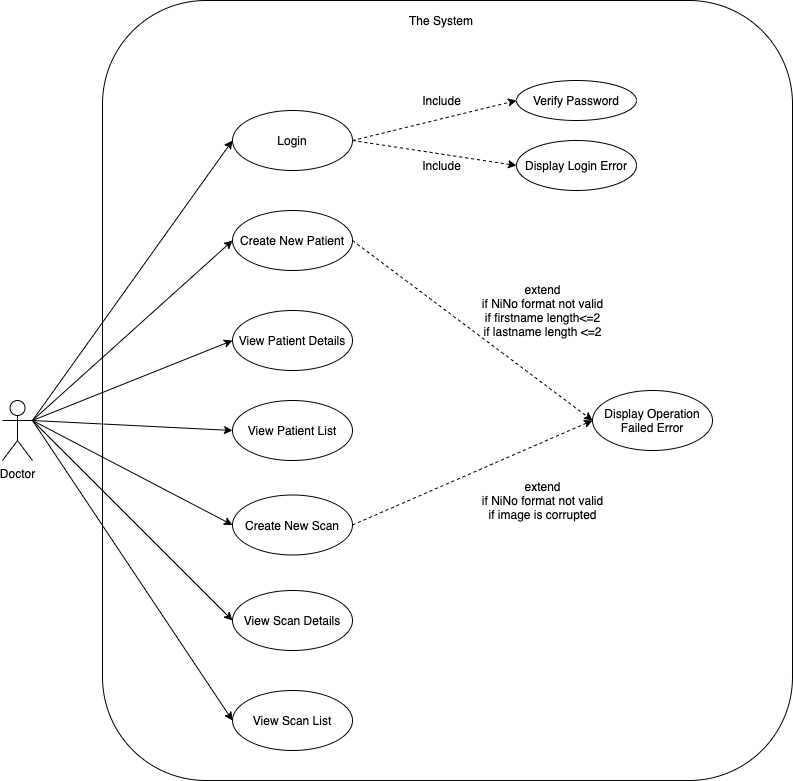
\includegraphics[scale=0.5]{figures/use-case}
				\fi
			\end{figure}
	\section{Non Functional Requirements}
		\label{non-functional-requirements}
		Nonfunctional requirements are the properties of the system; an comprehensive list of the agreed nonfuctional requirements is given below
		\begin{itemize}
			\item The system must be secure, as it handles the personal information of the patients
			\item The system should be reliable, as downtimes are affecting the hospital's performance 
			\item The system should be able to complete a prediction scan in a reasonable amount of time(1-10 mins)
		\end{itemize}
		


